%!TEX root = ../report.tex

\begin{document}
    \chapter{Experiment 02}
    \section{Deliverables}
    \begin{itemize}
        \item[] Write a report detailing your execution of the experiment, including all observations made while running the robot. Especially detail and visualize the observed robot end poses and report statistical precision of the observed end poses (combined data). Summarize your findings, does the observed behaviour of the robot matches your expectations? Your report should cover:
    \end{itemize}
    
    \begin{itemize}
        \item[1.] The program and parameters used to drive the robot
        \item[2.] Any observation made during the execution that may help one understand the outcome of the experiments (see also next week).
        \item[3.] The observed data (spread-out of the manually measured end poses) as Excel or LibreOffice Calc files (stored in .csv file format and structured as presented in table 3 (section A.2)). For the data collected by the control script (using the encoders’ readings) you can take already generated files from the EV3 brick.
        \item[4.] Visualization of the i) robot’s end poses (combined data from manual measurements), ii) complete robot’s paths (combined data from encoder measurements) as well as iii) visual documentation of all aspects of setup and execution you deem important. See figures 10, 11, 12 (section A.1) that show some examples on how the data can be visualized.
        \item[5.] Three videos showing robot’s behaviour during the experiment (one for each type of motion)
    \end{itemize}
    
    \section{Program \& Parameters}
    
    {
   \begin{minted}{python} 
    
    #!/usr/bin/env micropython

    from time import sleep, time
    import sys
    import math
    from ev3dev2.motor import LargeMotor, OUTPUT_A, OUTPUT_B, OUTPUT_C, OUTPUT_D, SpeedPercent,
    MoveTank
    from ev3dev2.sensor import INPUT_1, INPUT_2, INPUT_3, INPUT_4
    from ev3dev2.sound import Sound
    from ev3dev2.button import Button
    
    WHEEL_DIAMETER = 5.6  # cm
    MAIN_AXIS_LENGTH = 12.0  # cm
    
    buttons = Button()
    move = MoveTank(OUTPUT_A, OUTPUT_D)
    spkr = Sound()
    motor_1 = LargeMotor(OUTPUT_A)
    motor_2 = LargeMotor(OUTPUT_D)
    
    motor_1_path = []  # in rad
    motor_2_path = []  # in rad
    
    motor_1_path.append(motor_1.position)
    motor_2_path.append(motor_2.position)
    
    robot_orientation = 0.0  # in rad
    robot_position_x = 0.0  # in cm
    robot_position_y = 0.0  # in cm
    
    distance_traveled_wheel_1 = 0.0  # in cm
    distance_traveled_wheel_2 = 0.0  # in cm
    
    start_time = str(time()).split(".")[0]
    times_motor_1 = []
    times_motor_2 = []
    
    spkr.speak('Press a button')
    while True:
        if buttons.left:
            move.on_for_seconds(SpeedPercent(30), SpeedPercent(40), 2.2, block=False)
            file_name = 'left_' + start_time
    
        elif buttons.up:
            move.on_for_seconds(SpeedPercent(40), SpeedPercent(40), 2.2, block=False)
            file_name = 'up_' + start_time
    
        elif buttons.right:
            move.on_for_seconds(SpeedPercent(40), SpeedPercent(30), 2.2, block=False)
            file_name = 'right_' + start_time
    
        if (motor_1.is_running):
            motor_1_path.append((motor_1.position * math.pi) / 180.0)
            times_motor_1.append(time())
        if (motor_2.is_running):
            motor_2_path.append((motor_2.position * math.pi) / 180.0)
            times_motor_2.append(time())
    
        if (motor_1.is_holding and motor_2.is_holding):
            data_length = min(len(motor_1_path), len(motor_2_path))
    
            with open(file_name + '_both_motors_path.csv', "w") as f_wheels_path:
                header = 'motor_1_path_rad, motor_2_path_rad, time_motor_1, time_motor_2\n'
                f_wheels_path.write(header)
                for motor_1, motor_2, time_1, time_2 in zip(motor_1_path, \ 
                motor_2_path, times_motor_1, times_motor_2):
                    f_wheels_path.write(str(motor_1) + ', ' + str(motor_2) + ', ' +
                                        str(time_1) + ', ' + str(time_2) + '\n')  # in rad
    
            with open(file_name + '_robot_path.csv', "w") as f_robot_path:
                header = 'robot_position_x, robot_position_y, robot_orientation\n'
    
                f_robot_path.write(header)
                for i in range(data_length):
                    if i is 0:
                        distance_traveled_wheel_1 = (WHEEL_DIAMETER * math.pi * \
                        motor_1_path[0]) / (2 * math.pi)
                        distance_traveled_wheel_2 = (WHEEL_DIAMETER * math.pi * \
                        motor_2_path[0]) / (2 * math.pi)
                    else:
                        distance_traveled_wheel_1 = (WHEEL_DIAMETER * math.pi * \
                        (motor_1_path[i] - motor_1_path[i - 1])) /  (2 * math.pi)
                        distance_traveled_wheel_2 = (WHEEL_DIAMETER * math.pi * \
                        (motor_2_path[i] - motor_2_path[i - 1])) / (2 * math.pi)
    
                    delta_distance = (distance_traveled_wheel_1 + distance_traveled_wheel_2) / 2
                    delta_angle = (distance_traveled_wheel_1 - distance_traveled_wheel_2) / \
                    MAIN_AXIS_LENGTH
    
                    robot_orientation = robot_orientation + delta_angle
                    robot_position_x = robot_position_x + delta_distance * math.sin(robot_orientation)
                    robot_position_y = robot_position_y + delta_distance * math.cos(robot_orientation)
    
                    str_robot_position_x = str(robot_position_x)
                    str_robot_position_y = str(robot_position_y)
                    str_robot_orientation = str((math.pi / 2) - robot_orientation)
    
                    f_robot_path.write(str(str_robot_position_x + ', ' + str_robot_position_y +
                                           ', ' + str_robot_orientation + '\n'))
    
            spkr.speak('Motion completed')
            break
    
        # don't let this loop use 100% CPU
        sleep(0.001)
    
    \end{minted}
    }
    
    \section{Observations}
        \subsection{Before the experiment}
        \begin{itemize}
            \item Modifications were made to our initial measurement facility with the help of the pictures for the design of the measurement facility of Group 6.  It consisted of 2 pencils attached with tape to hinges made of some lego blocks. After finishing the assembly several points were noted and thus some modifications were needed: 
            \begin{itemize}
                \item [1.] It was observed that tape is bad for attaching the pencils because it does not exert sufficient pressure for a straight marking. So instead of tape we used cable ties as seen in Figure \ref{fig:cable ties}, \ref{fig:cable ties2}.
                
                \begin{figure}[!ht] 
                        \centering 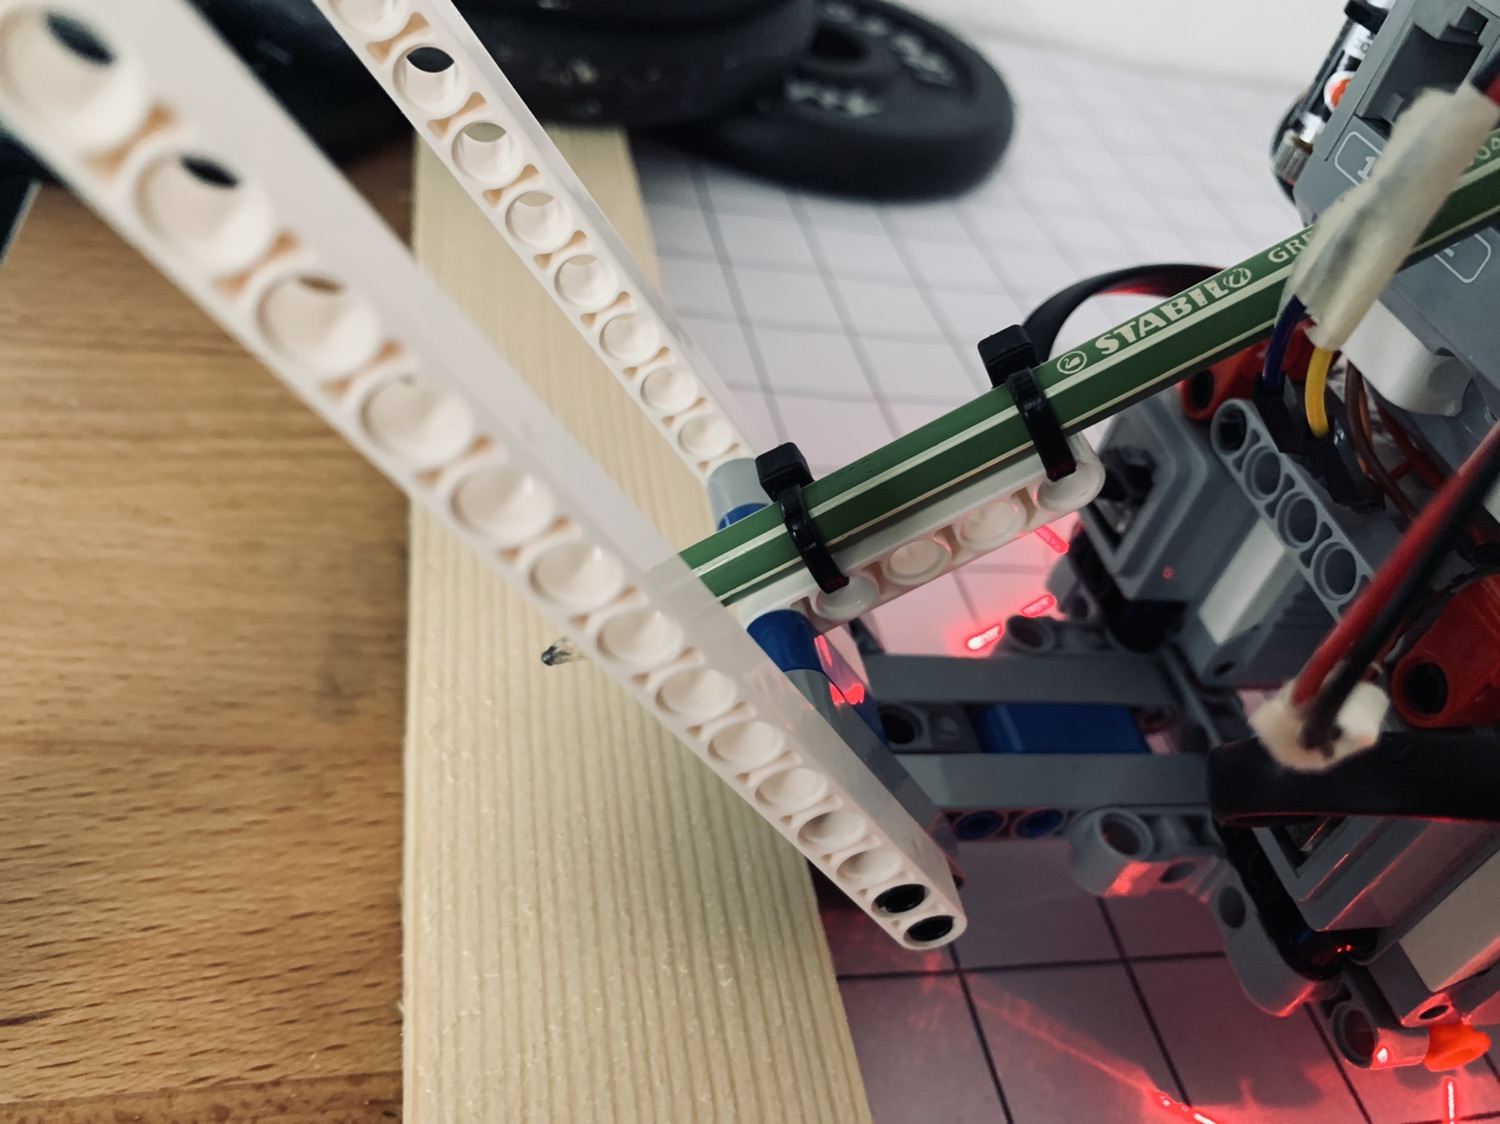
\includegraphics[scale=5.0]{"images/experiment_2/experiment-9.png"}
                        \caption{Attaching the pencils to Rosa}
                        \label{fig:cable ties}
                \end{figure}
                
                \begin{figure}[!ht] 
                        \centering 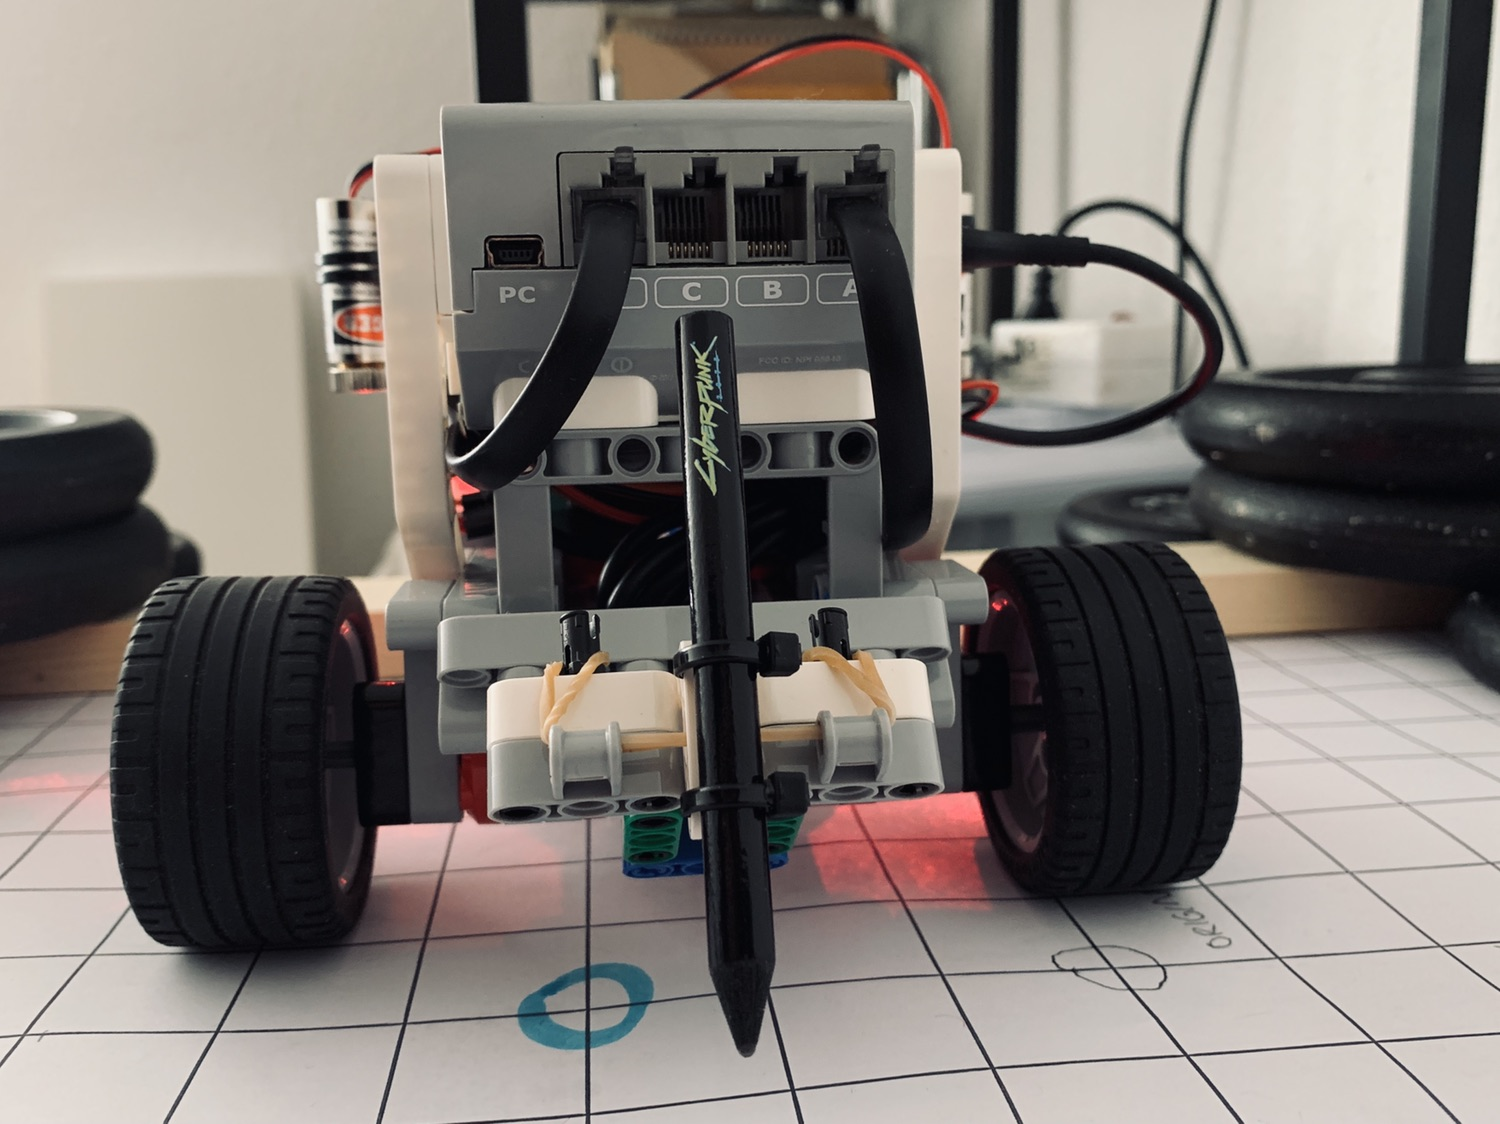
\includegraphics[scale=5.0]{"images/experiment_2/experiment-7.png"}
                        \caption{Attaching the pencils to Rosa}
                        \label{fig:cable ties2}
                \end{figure}
                
                \item[2.] The front hinge was wobbly. During testing it freed itself from the original locking mechanism. This is why we needed to develop a guidance system, which holds the pen in place with an elastic band and guides the pen evenly to the ground during marking as seen in Figure \ref{fig:elastic ties}.
                
                \begin{figure}[!ht] 
                        \centering 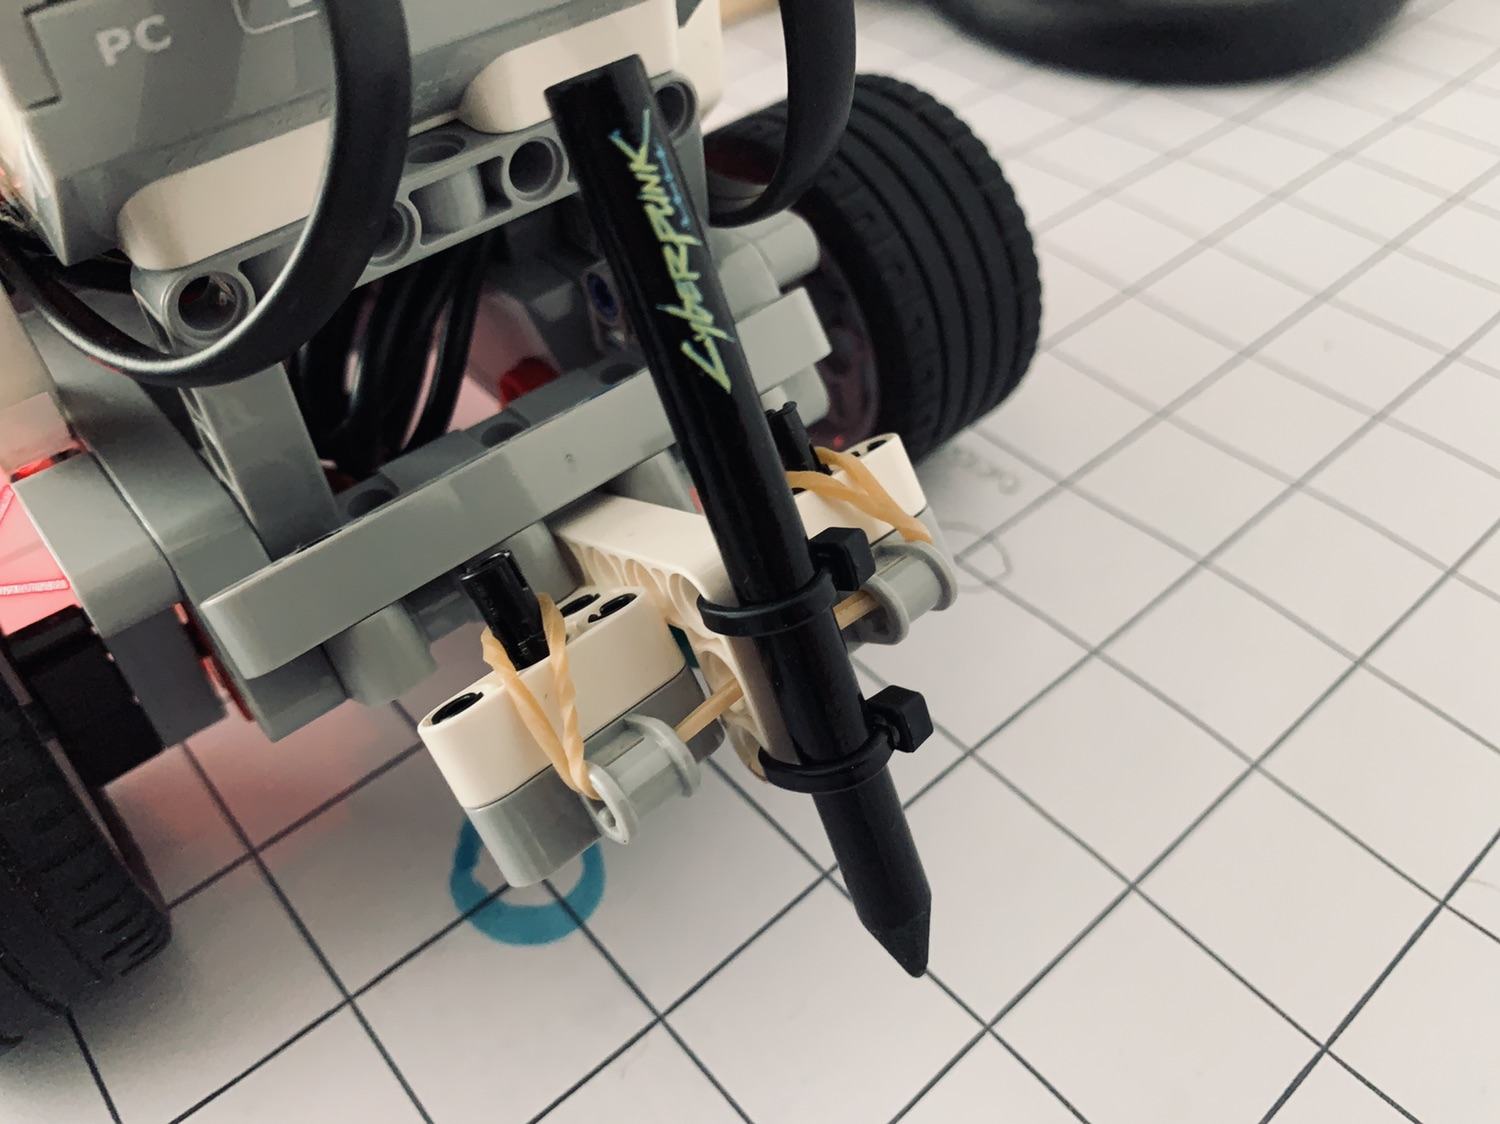
\includegraphics[scale=5.0]{"images/experiment_2/experiment-5.png"}
                        \caption{Elastic bands for guidance}
                        \label{fig:elastic ties}
                \end{figure}
                
                \item[3.] The design did not contain any help for resetting the robot to its start position. Since we did not need the lasers for marking positions any more, we attached them to the side of the robot's main corpus for easy resetting as seen in Figure \ref{fig:lasers}, \ref{fig:lasers2}. Another thing we did, was to use a wooden plank (Figure \ref{fig:wooden plank}) and some weights for creating a barrier to which we could roll the robot for a coarse positioning and the use the lasers for fast fine positioning.
                
                \begin{figure}[!ht] 
                        \centering 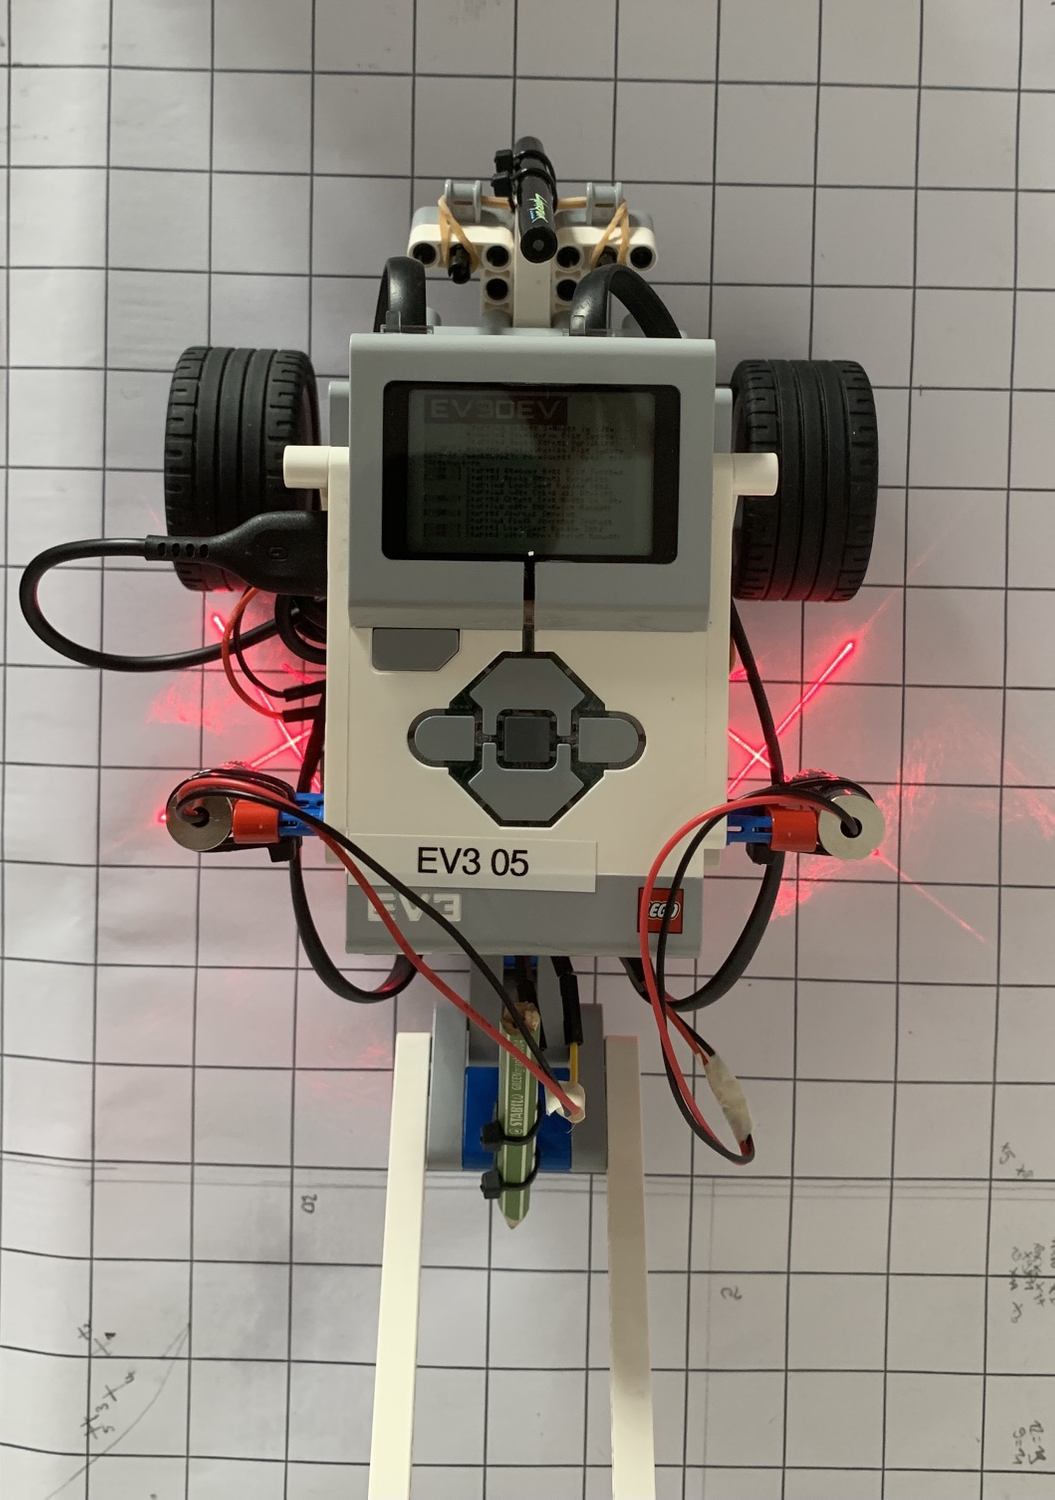
\includegraphics[scale=5.0]{"images/experiment_2/experiment-2.png"}
                        \caption{Lasers for ease of resetting position}
                        \label{fig:lasers}
                \end{figure}
                
                \begin{figure}[!ht] 
                        \centering 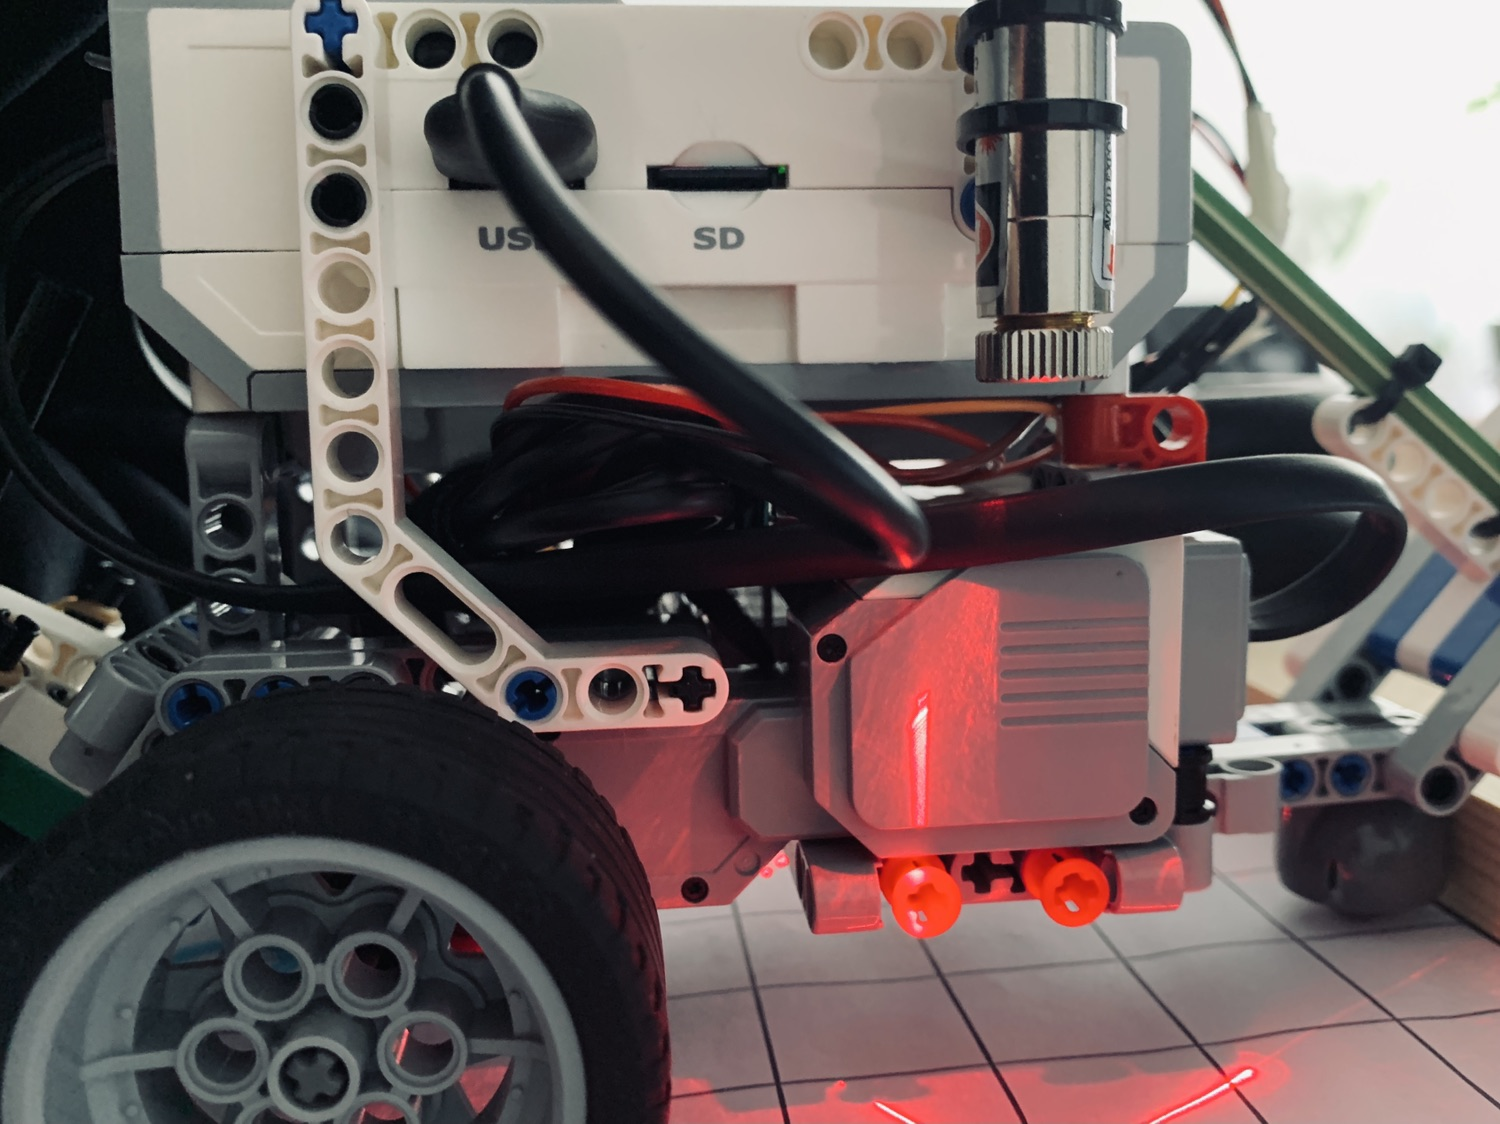
\includegraphics[scale=5.0]{"images/experiment_2/experiment-8.png"}
                        \caption{Lasers for ease of resetting position}
                        \label{fig:lasers2}
                \end{figure}
                
                \begin{figure}[!ht] 
                        \centering 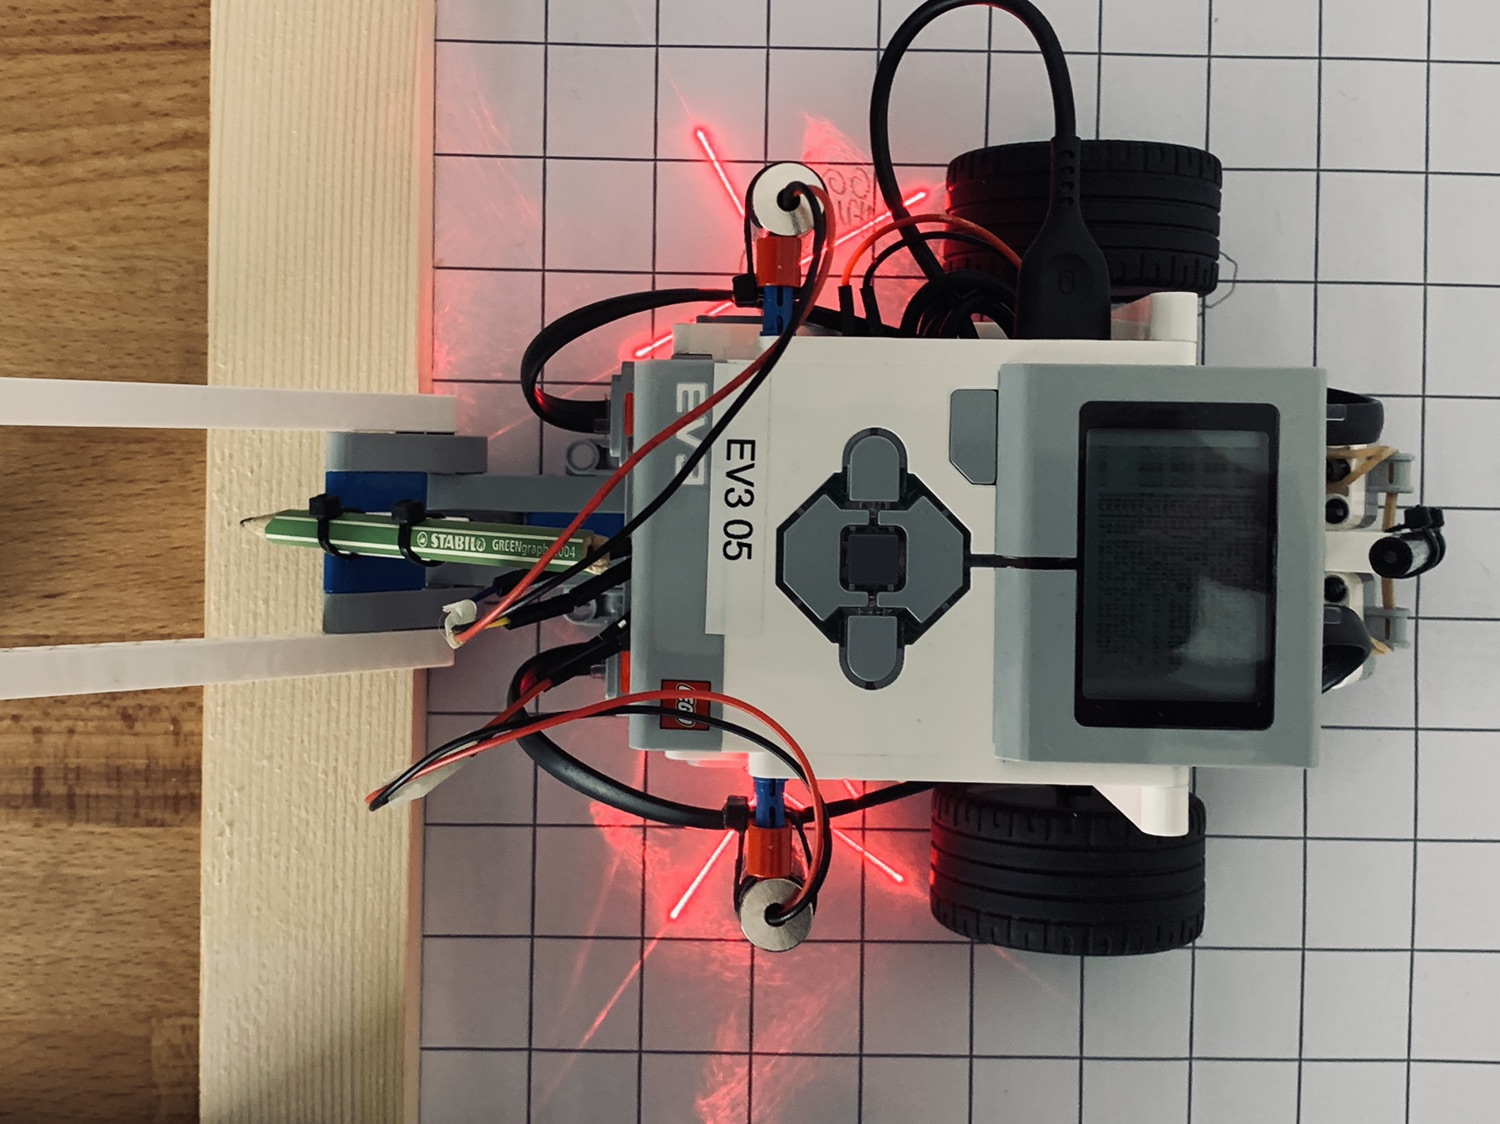
\includegraphics[scale=5.0]{"images/experiment_2/experiment-6.png"}
                        \caption{Wooden plank for creating a barrier}
                        \label{fig:wooden plank}
                \end{figure}
                
                \item[4.] The back hinge hold up fine, but it was a hassle to use the pen. So we attached some rails for easier one hand handling.
            \end{itemize}
            
        \subsection{During the experiment}
        \begin{itemize}
            \item[1.] Marking the positions with this new apparatus was a bit slower than using the lasers. The 2 pens had to be put down carefully. One hand had to hold the robot in position while the other hand pressed down the pen. As seen in Figure \ref{fig:grid marking}, this created a small dot and then carefully a small cross was put on the paper next to the experiments index. 
            
            \begin{figure}[!ht] 
                        \centering 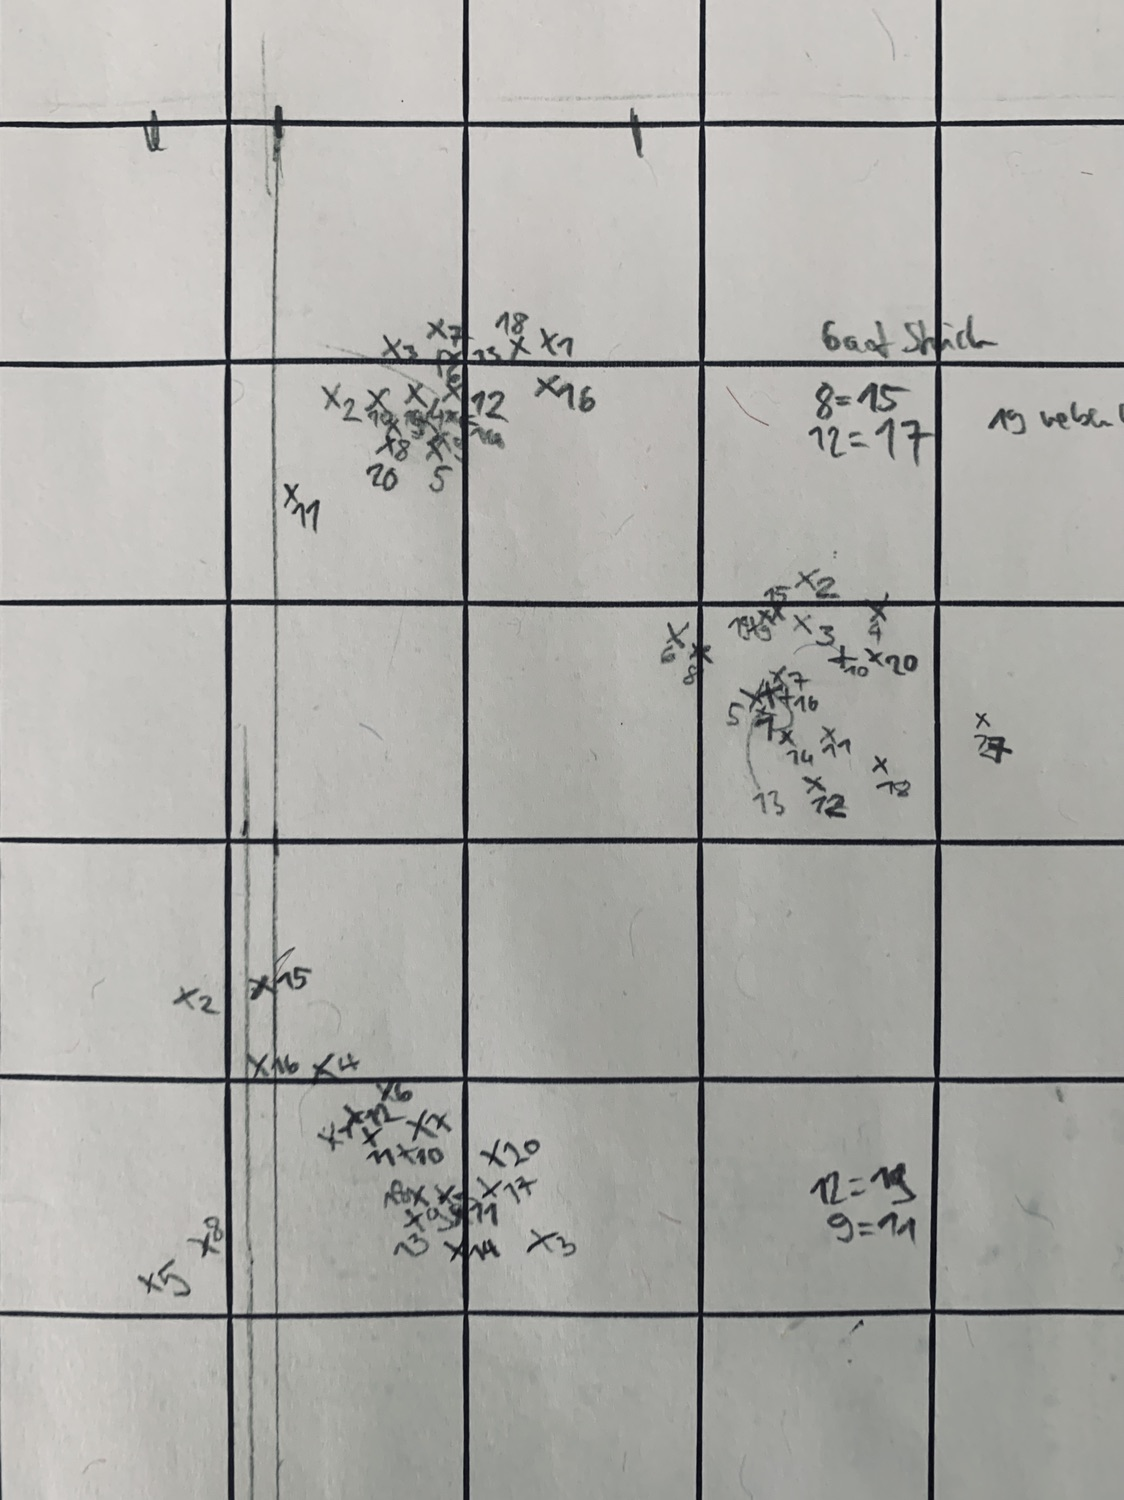
\includegraphics[scale=6.0]{"images/experiment_2/experiment.png"}
                        \caption{Making markings on the grid}
                        \label{fig:grid marking}
            \end{figure}
                 
            \item[2.] With the old design we only needed to put the cross on the paper and did not need to touch the robot at all (besides during resetting the robot). This had saved some time and prevented  accidentally moving the robot when using our old design.
            
            \item[3.] For keeping track of the robot's logs easily, we modified the control script to name each run in the following pattern: [up | left right][start\_time][robot\_path | both\_motors].csv
            
            \item[4.] After marking all 60 runs, we measured carefully the x and y position of each cross to a precision of 1 mm.
        \end{itemize}
        
        \subsection{After the experiment}
        \begin{itemize}
            \item[1.] The handwritten measures are written down into .csv files for further analyses. 
        \end{itemize}
        \end{itemize}
        
        
                
    
    {
    \section{Data Collected}
        \begin{itemize}
            \item Tables \ref{tab:forward-run}, \ref{tab: right-run}, \ref{tab:left-run} show the data collected during the forward, right and left runs respectively.
        \end{itemize}
        \begin{table}[h!]
        \centering
        \resizebox{\textwidth}{!}{%
        \begin{tabular}{|c|c|c|c|}
        \hline
        & X axis (cm) & Y axis(cm) & Orientation(deg) \\ \hline
        1 &  0.6         & 45.4       & -1.4262          \\ \hline
        2 & -1.25       & 45.85      & 1.6707           \\ \hline
        3 & -0.55       & 45.85      & 0.7102           \\ \hline
        4 & -0.65       & 46.55      & 0.7162           \\ \hline
        5 & 0.4         & 45.3       & -0.4755          \\ \hline
        6 & -0.2        & 44.45      & 1.9092           \\ \hline
        7 & 0.35        & 45.5       & 1.1885           \\ \hline
        8 & 0.2         & 44.7       & 0.9509           \\ \hline
        9 & -0.35       & 45.35      & -0.2368          \\ \hline
        10 & 0.05        & 46.15      & -0.7162          \\ \hline
        11 & 1.05        & 46.1       & -1.1885          \\ \hline
        12 & 1.15        & 46.8       & 0.6636           \\ \hline
        13 & 0.75        & 45.45      & -0.7102          \\ \hline
        14 & 1.05        & 45.65      & -1.1935          \\ \hline
        15 & -0.6        & 45.7       & 0.4876           \\ \hline
        16 & 0.45        & 45.65      & -0.2368          \\ \hline
        17 & 1.4         & 46.75      & -4.0856          \\ \hline
        18 & 1.55        & 46.6       & -2.1387          \\ \hline
        19 & -0.55       & 45.35      & 0.7102           \\ \hline
        20 & -0.35       & 46.85      & 1.2137           \\ \hline
        \end{tabular}%
        }
        \caption{Measurements taken in the forward run}
        \label{tab:forward-run}
        \end{table}
    
        \begin{table}[h!]
        \centering
        \resizebox{\textwidth}{!}{%
        \begin{tabular}{|c|c|c|c|}
        \hline
        & X axis (cm) & Y axis(cm) & Orientation(deg) \\ \hline
        1 & 15.2        & 35.3       & -57.4371         \\ \hline
        2 & 13.25       & 34.25      & -54.4342         \\ \hline
        3 & 16.5        & 36.85      & -60.8519         \\ \hline
        4 & 14.15       & 35.45      & -55.7763         \\ \hline
        5 & 15.95       & 34.35      & -51.2655         \\ \hline
        6 & 14.6        & 35.9       & -56.7752         \\ \hline
        7 & 15.2        & 36         & -58.7508         \\ \hline
        8 & 15.25       & 35.3       & -49.4248         \\ \hline
        9 & 16.1        & 35.8       & -58.9125         \\ \hline
        10 & 15.4        & 35.9       & -58.5023         \\ \hline
        11 & 15.15       & 35.95      & -59.8314         \\ \hline
        12 & 14.95       & 35.35      & -58.1726         \\ \hline
        13 & 16.35       & 36         & -58.7148         \\ \hline
        14 & 16.65       & 36.1       & -60.1063         \\ \hline
        15 & 13.2        & 35.05      & -54.4623         \\ \hline
        16 & 14.1        & 34.9       & -55.4419         \\ \hline
        17 & 16          & 36.55      & -59.6067         \\ \hline
        18 & 16          & 35.85      & -59.3646         \\ \hline
        19 & 15.05       & 35.45      & -58.0197         \\ \hline
        20 & 15.5        & 36.5       & -59.9863         \\ \hline
        \end{tabular}%
        }
        \caption{Measurements taken in the right run}
        \label{tab: right-run}
        \end{table}
        
        \begin{table}[h!]
        \centering
        \resizebox{\textwidth}{!}{%
        % \begin{adjustbox}{\columnwidth}
        \begin{tabular}{|c|c|c|c|}
        \hline
        & X axis (cm) & Y axis(cm) & Orientation(deg) \\ \hline
        1 & -13.05      & 37.85      & 54.8291          \\ \hline
        2 & -12.25      & 35.9       & 53.2759          \\ \hline
        3 & -12.7       & 36.45      & 53.6156          \\ \hline
        4 & -12.25      & 36.65      & 53.4711          \\ \hline
        5 & -11.5       & 37.15      & 51.87            \\ \hline
        6 & -12.6       & 36.95      & 53.2267          \\ \hline
        7 & -13.1       & 36.8       & 54.4906          \\ \hline
        8 & -11.7       & 36.65      & 51.87            \\ \hline
        9 & -11.5       & 37.4       & 51.0725          \\ \hline
        10 & -12.1       & 36.35      & 52.9356          \\ \hline
        11 & -10.85      & 35.95      & 50.6595          \\ \hline
        12 & -12.25      & 37.15      & 52.7885          \\ \hline
        13 & -12.65      & 37.2       & 52.8883          \\ \hline
        14 & -11.75      & 37.45      & 52.1036          \\ \hline
        15 & -11.8       & 36.7       & 51.9776          \\ \hline
        16 & -12.35      & 38.05      & 53.7592          \\ \hline
        17 & -12.3       & 37.35      & 52.1672          \\ \hline
        18 & -12.75      & 37.75      & 53.4711          \\ \hline
        19 & -11.85      & 37.1       & 51.8292          \\ \hline
        20 & -12         & 36.8       & 51.8292          \\ \hline
        \end{tabular}%
        }
        % \end{adjustbox}
        \caption{Measurements taken in the left run}
        \label{tab:left-run}
        \end{table}
    }
    
  {
    \section{Visualisations}
    
        \begin{figure}[!ht] 
            \centering 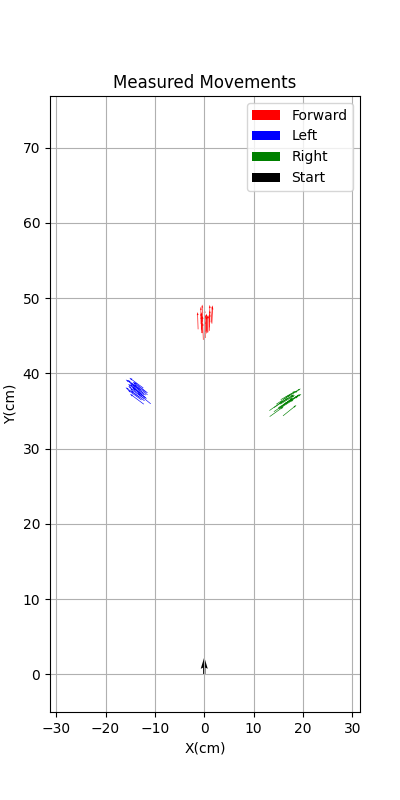
\includegraphics[scale=.70]{"images/experiment_2/1.end-poses.png"}
            \caption{Visualising the end poses from the manual measurements}
            \label{fig:end-poses}
        \end{figure}
        
        \begin{figure}[!ht] 
            \centering 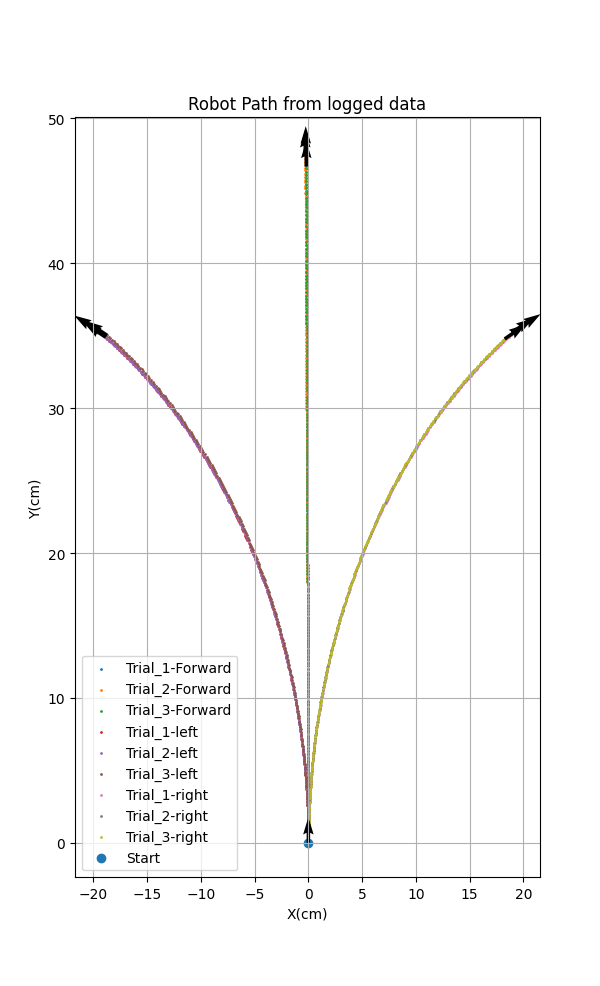
\includegraphics[scale=.60]{"images/experiment_2/2.path.png"}
            \caption{Visualising the paths from Encoder Data}
            \label{fig:path}
        \end{figure}
        
        \begin{figure}[!ht] 
            \centering 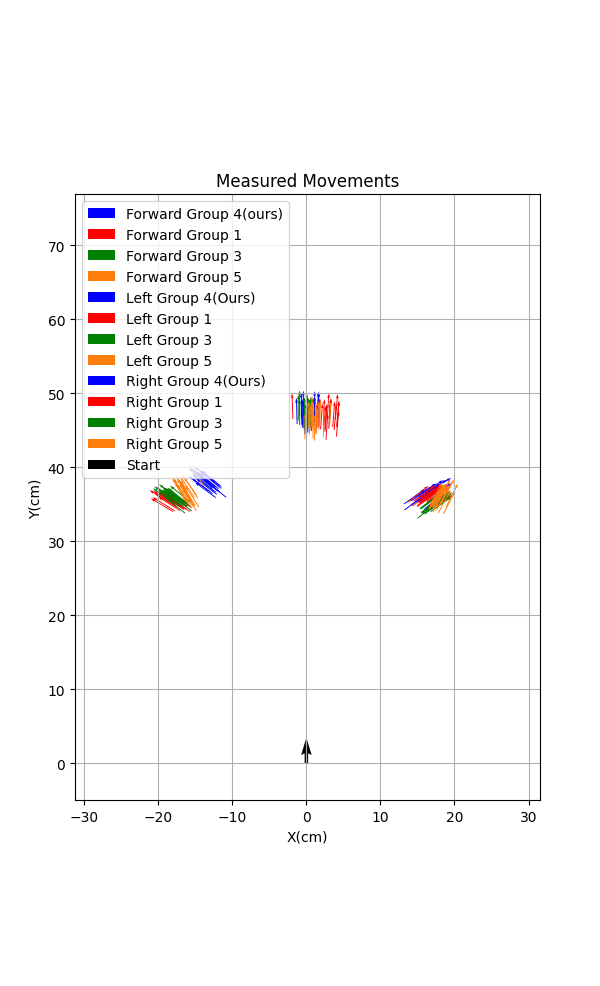
\includegraphics[scale=.60]{"images/experiment_2/3.merged-end-poses.png"}
            \caption{Visualising the end poses with manually measured data from all the groups}
            \label{fig:merged-end-poses}
        \end{figure}
    
        \begin{figure}[!ht] 
            \centering 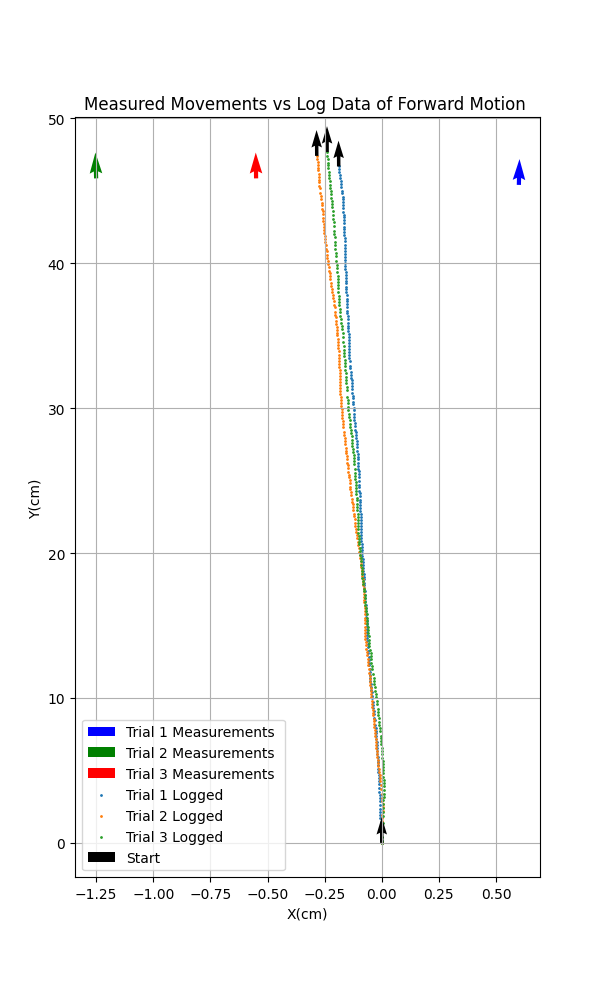
\includegraphics[scale=.60]{"images/experiment_2/Figure_forward.png"}
            \caption{Manual Measurement v/s Encoder Data for Forward Run}
            \label{fig:forward-manual-encoder}
        \end{figure}
        
        \begin{figure}[!ht] 
            \centering 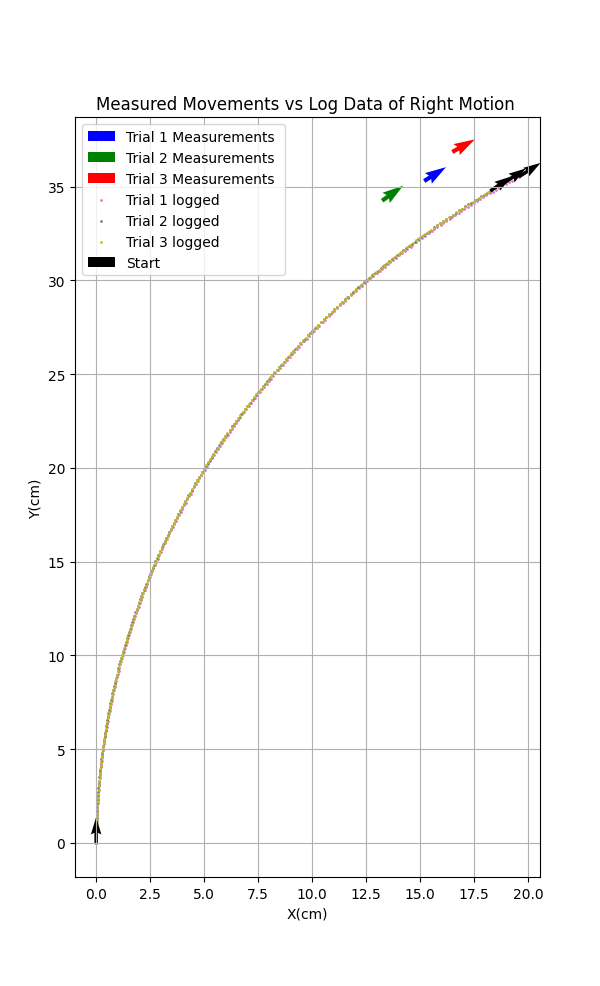
\includegraphics[scale=.60]{"images/experiment_2/Figure_right.png"}
            \caption{Manual Measurement v/s Encoder Data for Right Run}
            \label{fig:right-manual-encoder}
        \end{figure}
        
        \begin{figure}[!ht] 
            \centering 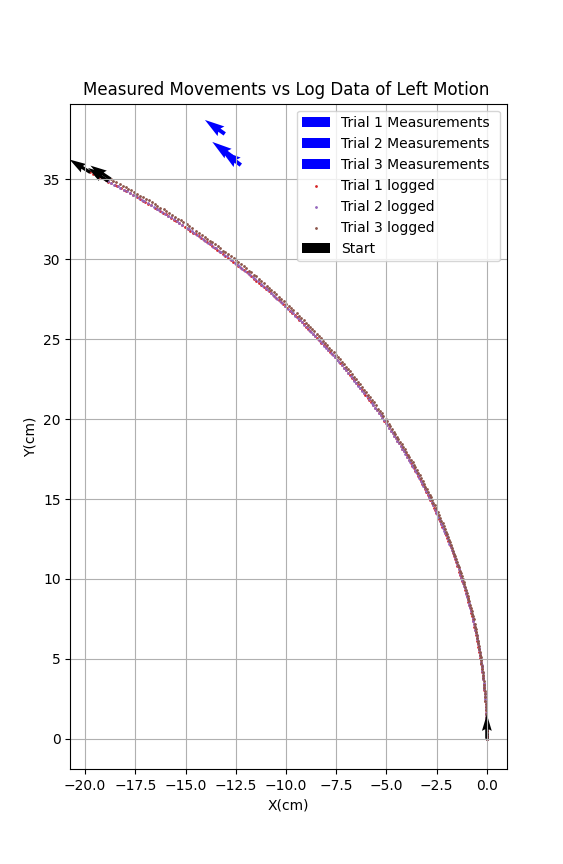
\includegraphics[scale=.60]{"images/experiment_2/Figure_left.png"}
            \caption{Manual Measurement v/s Encoder Data for Left Run}
            \label{fig:left-manual-encoder}
        \end{figure}
    }
    
    
    
\end{document}
